%----------------------------------------
% SECTION: From Lie groups to finite groups
%----------------------------------------
\section{From Lie groups to finite groups}
\label{sec:from_lie_groups_to_finite_groups}


\subsection{The Hilbert space}

\subsubsection{Basic construction}\label{sec:basic hilbert space}

In the Hamiltonian formulation of \ac{lgt}s \cite{KogSuss, Osborne, ZoharBurrello}, time is continuous while the $d$ spatial dimensions are discretized into a hypercubic lattice.
Classically, we assign a group element $g \in G$ to each spatial lattice link, where $G$ is the gauge group.
In the Lie group case, one would typically write $U_\mu(x) = \exp{(iA_\mu(x))} \in G$ for the gauge field variable assigned to the lattice link between points $x$ and $x + \hat{\mu}$, where $A_\mu(x)$ is the vector potential.
Links are oriented, and if a link is traversed in the opposite orientation, then $g$ is replace with $g^{-1}$.
Note that finite groups have no Lie algebras, so we work with group-valued quantities as far as possible.
In what follows, we write $g \in G$ for a group element indifferently for both finite and Lie groups $G$.
Since classically we have a group element $g$ on each lattice link, in the quantum theory the states in the Hilbert space of each link are given by \cite{Osborne}
\begin{equation}
    \ket{\psi}=\int dg \, \psi(g)\ket{g} \ ,
\end{equation}
where $\{\ket{g}\}$ is the group element orthonormal basis, consisting of one state $\ket{g}$ per group element $g$; it can be though of as a \say{position basis} on the group.
The wavefunction $\psi(g)$ is square-integrable with respect to the Haar measure.
For a finite group, the Haar measure is simply a sum over group elements, $\int dg = \sum_g$.
The Hilbert space on each link can then be identified with $L^2(G)$, i.e. the space of square-integrable functions on $G$ \cite{Osborne}, while for a finite group it is simply the \textit{group algebra} $\C[G]$, which is the complex vector space spanned by the group element basis.
The overall Hilbert space is then given by the tensor product $\mathcal{H} = \bigotimes_{\mathrm{links}} L^2(G)$, or $\mathcal{H} = \bigotimes_{\mathrm{links}} \C[G]$.
Note that for a finite group, $\C[G]$ has finite dimension, because it is spanned by the finitely-many group element states $\{\ket{g}\}$.
Therefore the Hilbert space on each link is finite-dimensional and $\mathcal{H}$ is finite-dimensional on a finite lattice; its dimension is in fact given by $\abs{G}^L$ where $L$ is the number of lattice links.
For a Lie group, on the other hand, we have infinitely many basis states $\{\ket{g}\}$ and therefore the Hilbert space is infinite-dimensional \textit{on each link}.

In the Hamiltonian formulation of gauge theories, the statement that the theory is invariant under gauge transformations translates at the level of the Hilbert space by restricting the allowed states only to those which are gauge-invariant.
In particular, on the single-link Hilbert space one can define left and right \say{translation} operators, in the analogy where $\{\ket{g}\}$ is a position basis in group space \cite{ZoharBurrello},
\begin{equation}
    \label{eq:regular representations}
    L_g \ket{h} = \ket{gh} \ , \quad \quad R_g \ket{h} = \ket{gh^{-1}} \ .
\end{equation}
A local gauge transformation is given by a choice of group element $g_x \in G$ at every site $x$ of the lattice \cite{Osborne}.
This acts on the overall Hilbert space $\mathcal{H} = \bigotimes_{\mathrm{links}} L^2(G)$ or $\mathcal{H} = \bigotimes_{\mathrm{links}} \C[G]$ via the operator
\begin{equation}
    \label{eq:gauss law operator}
    \mathcal{G}(\{g_x\}) = \bigotimes_{l=\expval{xy} \in \mathrm{links}} L_{g_{x}} R_{g_y} \ ,
\end{equation}
where $\{g_x\}$ is an arbitrary choice of group elements $g_x$ at each lattice site $x$ and the link $l$ connects the points $x$ and $y$.
In other words, on each link the gauge transformation is given on basis elements by the familiar $\ket{g_l} \to \ket{g_x g_l g_y^{-1}}$.
The only physical states are those which satisfy the so-called \say{Gauss' law} constraint \cite{KogSuss, Osborne, Tong}
\begin{equation}
    \label{eq:lattice gauss law}
    \mathcal{G}(\{g_x\}) \ket{\psi}=\ket{\psi} \ ,
\end{equation}
for any possible choice of local assignments $\{g_x\}$ of group variables to lattice sites.
The states which satisfy eq.~\eqref{eq:lattice gauss law} form the physical, gauge-invariant Hilbert space $\mathcal{H}_\mathrm{phys}$.
Note that the condition eq.~\eqref{eq:lattice gauss law} only involves group-valued quantities and is thus valid for both Lie groups and finite groups.
In the case of finite groups, the condition simplifies because it is sufficient to impose invariance against a set of generators of the finite group.

One can also straightforwardly include matter fields such as fermion fields which live on each lattice site.
Under a gauge transformation, they transform as $\Psi(x) \to g_x \Psi(x)$.
Since these always have a finite Hilbert space, they do not additional issues for quantum simulation and we focus instead on the pure gauge theory.

\subsubsection{The representation basis and the Peter-Weyl theorem}\label{sec:representation basis}

It turns out to be fruitful to introduce a different basis of the overall Hilbert space $\mathcal{H}$, \say{dual} to the group element basis.
The operators $L_g$ and $R_g$ introduced in eq.~\eqref{eq:regular representations} are unitary representations of $G$, known as the \textit{left} and \textit{right regular} representations \cite{Serre, KnappLieGroups}.
This is because $L_g L_h = L_{gh}$ and $(L_g)^{-1}=L_{g^{-1}}=(L_g)^\dagger$, as can be explicitly checked by acting on the group element basis, and the same holds for $R$.
Their representation theory leads to the Peter-Weyl theorem \cite{KnappLieGroups, Osborne, marianithesis}, which states that for a finite or compact Lie group $G$,
\begin{equation}
    \label{eq:peterweyl}
    L^2(G) = \bigoplus_{j \in \Sigma} V_j^* \otimes V_j \ ,
\end{equation}
where $j$ is a label for the irreducible representations (irreps) of $G$, and $\Sigma$ is the set of all irreps of $G$.
For finite groups $L^2(G)$ is replaced, as usual, with $\C[G]$.
Here $V_j$ is the representation vector space corresponding to representation $j$ and $V_j^*$ its dual vector space.
For both compact Lie groups and finite groups the irreps are finite-dimensional and can be chosen to be unitary.
For a finite group, $\Sigma$ is a finite set, while it is countably infinite for a compact Lie group \cite{KnappLieGroups, Serre}.
In terms of the Peter-Weyl decomposition, the left and right regular representations take a particularly simple form \cite{marianithesis},
\begin{equation}
    \label{eq:translations peter weyl}
    L_g R_h = \bigoplus_j \rho_j(g)^* \otimes \rho_j(h) \ ,
\end{equation}
where $\rho_j$ is the matrix of the $j$th irrep of $G$.
The individual action of either $L_g$ or $R_h$ may be obtained by setting either $g$ or $h$ to the identity.
Eq.~\eqref{eq:translations peter weyl} is especially useful because, as we will see in Section \ref{sec:physical Hilbert space}, it simplifies the action of the Gauss' law constraint eq.~\eqref{eq:lattice gauss law}.

The Peter-Weyl theorem provides an alternative basis for the single-link Hilbert space.
For each irrep $j$ one chooses appropriate bases for $V_j^*$ and $V_j$, which we denote $\{\ket{jm}\}$ and $\{\ket{jn}\}$ respectively, where $1 \leq m,n \leq \dim{j}$.
Here $\dim{j} \equiv \dim{V_j}$ is the dimension of the representation.
On each representation subspace, we use the shorthand notation $\ket{jmn} \equiv \ket{jm} \otimes \ket{jn}$.
Then the \say{representation basis} for $L^2(G)$ or $\C[G]$ is given by the set $\{\ket{jmn}\}$ for all $j \in \Sigma$ and $1 \leq m,n \leq \dim{j}$.
In terms of the group element basis, one has \cite{ZoharBurrello}
\begin{equation}
    \label{eq:change of basis}
    \expval{g|jmn}= \sqrt{\frac{\mathrm{dim}(j)}{\abs{G}}} \left[\rho_j(g)\right]_{mn} \ ,
\end{equation}
where the bases $\{\ket{jm}\}$, $\{\ket{jn}\}$ are chosen so that $\rho_j$ is unitary.
It should be emphasized that eq.\eqref{eq:change of basis} is valid for both finite and compact Lie groups; $\abs{G}$ is either the order of the finite group or the volume $\abs{G}\equiv\int dU\, 1$ given by the possibly unnormalized Haar measure \cite{Osborne, marianithesis}.
It is a basic result of the representation theory of finite groups that $\sum_j \pqty{\dim{j}}^2 = \abs{G}$, which ensures that the group element basis and the representation basis have the same number of states \cite{Serre}.

Since every group admits a trivial, one-dimensional irrep with $\rho(g)\equiv 1$, we always have a singlet representation state $\ket{0}$, which may be extended to the whole lattice to form the \say{electric ground state} $\ket{0_E}$,
\begin{equation}
    \label{eq:electric ground state}
    \ket{0_E} = \bigotimes_{l \in \mathrm{links}} \ket{0}_l \ , \quad \quad \ket{0}=\frac{1}{\sqrt{\abs{G}}} \sum_g \ket{g} \ ,
\end{equation}
where we used eq.\eqref{eq:change of basis} to express $\ket{0}$ in the group element basis.
We have summarized the representation theory of some groups of interest in Appendix \ref{sec:some groups of interest}.
In the specific case of the group $\Z_N$, the representations are all one-dimensional because $\Z_N$ is Abelian and therefore $m=n=1$ and can be omitted.
The group elements are $\{1, g, g^2, \ldots, g^{N-1}\}$ and the irreps are simply $\rho_j (g^k) = \omega_N^{kj}$ for $j = 0,1,\ldots, N-1$, with $\omega_N= e^{2\pi i /N}$.
The bases $\{\ket{g^k}\}$ and $\{\ket{j}\}$ are related by
\begin{equation}
    \ket{j} = \sum_{k=0}^{N-1}  \ket*{g^k} \braket*{g^k}{j} = \frac{1}{\sqrt{N}}\sum_{k=0}^{N-1} \omega_N^{kj} \ket*{g^k} \ ,
\end{equation}
which is just the discrete Fourier transform.
In the case of the dihedral groups $D_4$ with $8$ elements, we have four one-dimensional representations, each of which spans a one-dimensional subspace of $\C[G]$.
We then have a two-dimensional representation which spans a $2^2=4$ dimensional subspace of $\C[G]$ through the four basis elements $\ket{jmn}$ for $1 \leq m, n \leq 2$.

\subsection{The Hamiltonian}

\subsubsection{Basic construction}\label{eq:hamiltonian basic construction}

The Hamiltonian for a Yang-Mills gauge theory on the lattice takes the form \cite{KogSuss, ZoharBurrello}
\begin{equation}
    \label{eq:generic hamiltonian}
    H = \lambda_E \sum_{l \in \mathrm{links}} h_E(g_l) + \lambda_B \sum_{\square} h_B(g_\square) \ ,
\end{equation}
where $h_E$ depends only on each lattice link, while $h_B$ depends on the lattice plaquettes $\square$ and $g_\square = g_1 g_2 g_3^{-1} g_4^{-1}$ is the product of the four link variables in a lattice plaquette with the appropriate orientation.
It is also possible to add matter fields such as fermions, but since this does not pose any further difficulty than in the usual Lie group case, we focus here on the pure gauge theory.

In the Lie group case, the electric and magnetic Hamiltonians form the so-called Kogut-Susskind Hamiltonian where \cite{KogSuss, Osborne}
\begin{equation}
    \label{eq:kog suss hE hB}
    h_E = \sum_{a} \pqty{\hat{\ell}^a_L}^2 \ , \quad \quad \quad \quad h_B = \dim{\rho} - \Re \tr{\rho(g_\square)} \ ,
\end{equation}
where $\rho$ is the fundamental representation of $\SU(N)$, $a$ is a color index and $\hat{\ell}^a_L$ is the infinitesimal generator of left-translations, i.e. the Lie algebra representation corresponding to $L_g$.
As such, it satisfies $L_{e^{iX}} = \exp{\pqty{i \hat{\ell}_L(X)}}$ \cite{Osborne}.
As the group element basis may be thought of as a \say{position basis} in group space, the infinitesimal generator of translations $\hat{\ell}_L^a$ may be thought of as a \say{momentum} operator in group space.
Then the electric Hamiltonian $h_E$, which is the sum of the squares of the \say{momenta} in all directions, is a Laplacian in group space.
Applying the Peter-Weyl decomposition eq.~\eqref{eq:translations peter weyl} to $\hat{\ell}_L^a$, one finds that \cite{Osborne,marianithesis}
\begin{equation}
    \label{eq:laplacian decomposition}
    h_E = \sum_{a} \pqty{\hat{\ell}^a_L}^2 = \sum_{jmn} C(j) \ket{jmn}\bra{jmn} \ ,
\end{equation}
where $C(j)$ is the quadratic Casimir operator, which depends only on the representation $C(j)$.
For $\U(1)$, for example $C(j)=j^2$, while for $\SU(2)$ one finds $C(j) = j(j+1)$.
We note that the magnetic Hamiltonian depends only on group-valued quantities and is therefore well-defined for both Lie groups and finite groups.
On the other hand, the electric Hamiltonian depends on the infinitesimal Lie algebra through $\hat{\ell}_L^a$ and therefore the definition does not extend to finite groups.
The decomposition eq.~\eqref{eq:laplacian decomposition} is well-defined also for finite groups, but one must leave the coefficients $C(j)$ unsatisfactorily unspecified because finite groups do not have a Casimir operator \cite{ZoharBurrello}.

If one thinks of a finite group as a natural discretization of some parent Lie group, the natural choice of electric Hamiltonian is a discrete Laplacian on the finite group.
The geometric structure of a finite group is that of a graph, with group elements as vertices and the group operation defining the edges.
This is called a \textit{Cayley graph}.
The discrete Laplacian on the finite group is then naturally given by the graph Laplacian of the Cayley graph.
This choice also preserves the interpretation of the electric Hamiltonian as a quantum-mechanical rotor in group space \cite{KogSuss}.
We explain the construction of the finite group Laplacian in detail in Section \ref{sec:finitegrouplaplacian}, and the resulting Hamiltonian takes the form of eq.~\eqref{eq:generic hamiltonian} with
\begin{equation}
    \label{eq:generalized ym hamiltonian}
    h_E = \sum_{g \in \Gamma} (1-L_g)  \ , \quad \quad \quad \quad h_B= h_B (g_\square) \ ,
\end{equation}
where $\Gamma \subset G$ is a subset of the group (\textit{not} a subgroup) such that
\begin{enumerate}
    \item $1 \not \in \Gamma$, i.e. $\Gamma$ doesn't contain the identity element.
    \item $\Gamma^{-1}=\Gamma$, i.e. it is invariant under inversion of group elements.
In other words, if $g \in \Gamma$, then $g^{-1} \in \Gamma$ also.
    \item $g \Gamma g^{-1} = \Gamma$, i.e. it is invariant under conjugation.
In other words, $\Gamma$ is a union of conjugacy classes of $G$.
\end{enumerate}
These conditions on $\Gamma$ ensure that the electric Hamiltonian is gauge-invariant.
On the other hand, as usual, the magnetic term is gauge-invariant as long as $h_B$ is any real function such that $h_B(g_1 g_\square g_1^{-1})=h_B(g_\square)$ for any $g_1 \in G$.
As explained in Section \ref{sec:action formulation}, the Hamiltonian eq.~\eqref{eq:generalized ym hamiltonian} includes as a special case the transfer-matrix Hamiltonian obtained in \cite{TransferMatrixFiniteGroup} which consists in a certain specific choice of subset $\Gamma$.
The choice of $\Gamma$ is in fact not unique, a fact which we will also discuss in later sections.

While the magnetic Hamiltonian $h_B$ is diagonal in the group element basis, the electric Hamiltonian $h_E$ is diagonal in the representation basis, and in fact
\begin{equation}
    \label{eq:electric hamiltonian rep basis}
    h_E = \sum_{jmn} h_E(j) \ket{jmn}\bra{jmn} \ , \quad \quad \quad h_E(j)=\abs{\Gamma} - \frac{1}{\dim{j}} \sum_{g \in \Gamma} \chi_j(g)\ ,
\end{equation}
where $\abs{\Gamma}$ is the number of elements in $\Gamma$ and $\chi_j$ is the character of the irrep labelled $j$.
The electric Hamiltonian may be interpreted as an \say{on-link} hopping term withing group space; in fact, up to a constant, it may be written as $h_E = \sum_{g \in \Gamma} \sum_{h \in G} \ket{gh}\bra{h}$ and it favours each link to sit in the electric ground state eq.~\eqref{eq:electric ground state}, which is fully delocalized in group space.
On the other hand, the magnetic term is a plaquette-based potential which pushes plaquettes close to the identity.
The competition between the two non-commuting terms gives rise to non-trivial dynamics.

We would like to emphasize that the description of the electric Hamiltonian $h_E$ in eq.~\eqref{eq:generalized ym hamiltonian} as the graph Laplacian of the Cayley graph associated with the group is not simply an interesting analogy, but also a tool which may be used to extract information on the Hamiltonian itself.
As an example, we note the well-known fact that the smallest eigenvalue of a graph Laplacian is always zero (given by the trivial representation state eq.~\eqref{eq:electric ground state}) and its degeneracy equals the number of connected components of the graph \cite{spectralgraphtheory}.
Moreover, it is not hard to show that the if $\Gamma$ does not generate the group $G$, but rather only a subset $\expval{\Gamma} < G$, then the Cayley graph splits into connected components which are identified with the cosets of $\expval{\Gamma}$ in $G$.
The number of such components, and therefore the degeneracy of the electric ground state, is given by $\abs{G}/\abs{\expval{\Gamma}}$.
If, instead, $\Gamma$ generates the whole group, then the electric Hamiltonian is not degenerate.
For more details, see Appendix \ref{sec:laplacian degeneracy}.
The degeneracy of the electric ground state is not only an important feature of the theory, but also technically important for ground state preparation and adiabatic quantum simulation.
As we will already at the end of Section \ref{sec:finitegrouplaplacian}, this can happen already for the dihedral group $D_4$.
In general, this can also occur with the choice of $\Gamma$ arising from the transfer-matrix formulation of Wilson action, as described in Section \ref{sec:action formulation}.
For example, in the permutation group $G=S_5$, starting from the Wilson action in the six-dimensional representation of $S_5$, one finds $\Gamma$ to be the conjugacy class of the $5$-cycles; then $\expval{\Gamma}$ generates the subgroup $A_5$ and since $\abs{S_5}/\abs{A_5}=2$, the electric Hamiltonian ground state is two-fold degenerate, with the ground states spanned by the two representation states corresponding to the one-dimensional representations.


\begin{figure}[t]
    \centering
    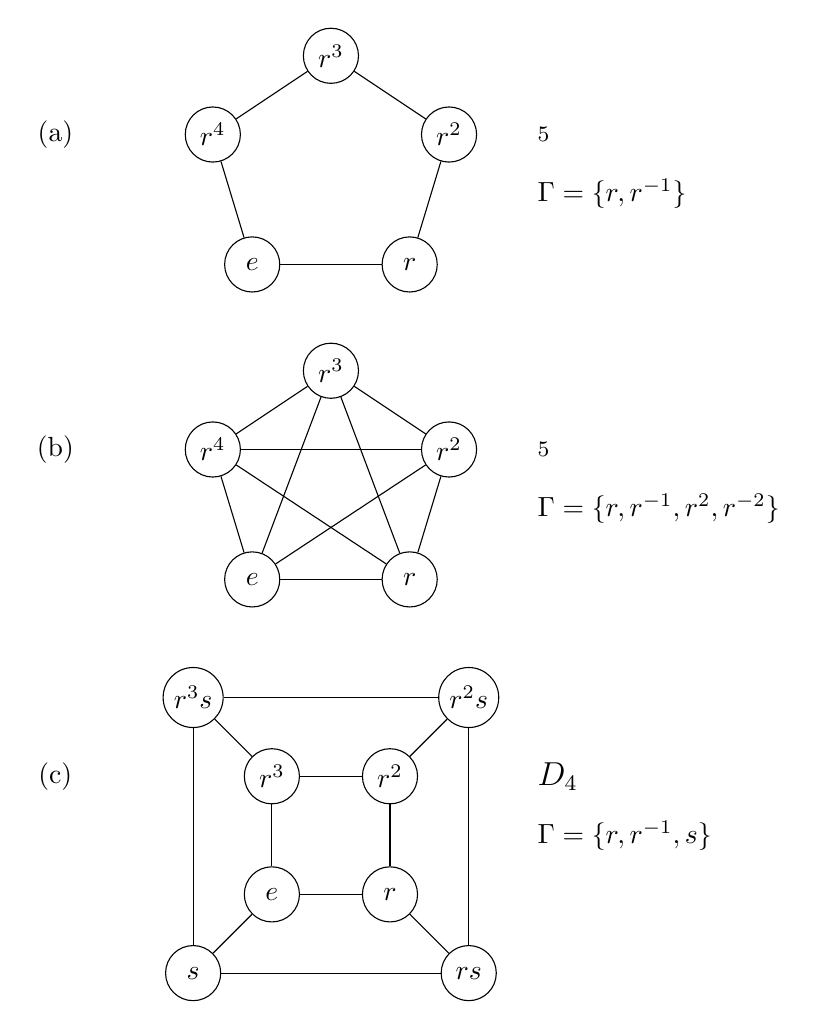
\begin{tikzpicture}[
    cell/.style = {shape=circle, draw=black, minimum width=0.7cm, inner sep=2pt}
    ]

    \node[cell] (g0) at (0,    0)    {$e$};
    \node[cell] (g1) at (2,    0)    {$r$};
    \node[cell] (g2) at (2.5,  1.65) {$r^2$};
    \node[cell] (g3) at (1,    2.65) {$r^3$};
    \node[cell] (g4) at (-0.5, 1.65) {$r^4$};

    \path [-] (g0) edge (g1);
    \path [-] (g1) edge (g2);
    \path [-] (g2) edge (g3);
    \path [-] (g3) edge (g4);
    \path [-] (g4) edge (g0);

    \begin{scope}[yshift=-4cm]
        \node[cell] (r0) at (0,    0)    {$e$};
        \node[cell] (r1) at (2,    0)    {$r$};
        \node[cell] (r2) at (2.5,  1.65) {$r^2$};
        \node[cell] (r3) at (1,    2.65) {$r^3$};
        \node[cell] (r4) at (-0.5, 1.65) {$r^4$};

        \path [-] (r0) edge (r1);
        \path [-] (r0) edge (r2);
        \path [-] (r1) edge (r2);
        \path [-] (r1) edge (r3);
        \path [-] (r2) edge (r3);
        \path [-] (r2) edge (r4);
        \path [-] (r3) edge (r4);
        \path [-] (r3) edge (r0);
        \path [-] (r4) edge (r0);
        \path [-] (r4) edge (r1);
    \end{scope}

    \begin{scope}[yshift=-8cm, xshift=0.25cm]
        \node[cell] (dih e)   at (0,   0)   {$e$};
        \node[cell] (dih r)   at (1.5, 0)   {$r$};
        \node[cell] (dih r2)  at (1.5, 1.5) {$r^2$};
        \node[cell] (dih r3)  at (0,   1.5) {$r^3$};
        \node[cell] (dih s)   at (-1,  -1)  {$s$};
        \node[cell] (dih rs)  at (2.5, -1)  {$rs$};
        \node[cell] (dih r2s) at (2.5, 2.5) {$r^2s$};
        \node[cell] (dih r3s) at (-1,  2.5) {$r^3s$};

        \path [-] (dih e) edge (dih r);
        \path [-] (dih e) edge (dih s);

        \path [-] (dih e) edge (dih r3);
        \path [-] (dih s) edge (dih r3s);

        \path [-] (dih r) edge (dih r2);
        \path [-] (dih r) edge (dih rs);

        \path [-] (dih r2) edge (dih r3);
        \path [-] (dih r2) edge (dih r2s);

        \path [-] (dih r3) edge (dih r3s);
        \path [-] (dih s) edge (dih rs);

        \path [-] (dih rs) edge (dih r2s);
        \path [-] (dih r2s) edge (dih r3s);
    \end{scope}

    % Group labels
    \node[align=left, anchor=west, font=\large] at (3.5, 1.65) {$\Z_5$};
    \node[align=left, anchor=west, font=\large] at (3.5, -2.35) {$\Z_5$};
    \node[align=left, anchor=west, font=\large] at (3.5, -6.5) {$D_4$};

    % Set labels
    \node[align=left, anchor=west] at (3.5, 0.9) {$\Gamma = \{r, r^{-1}\}$};
    \node[align=left, anchor=west] at (3.5, -3.1) {$\Gamma = \{r, r^{-1}, r^2, r^{-2}\}$};
    \node[align=left, anchor=west] at (3.5, -7.25) {$\Gamma = \{r, r^{-1}, s\}$};

    % Figure labels
    \node[font=\normalsize] at (-2.5, 1.65)  {(a)};
    \node[font=\normalsize] at (-2.5, -2.35) {(b)};
    \node[font=\normalsize] at (-2.5, -6.5)    {(c)};
\end{tikzpicture}

    \caption[Examples of Cayley graphs]{%
        Examples of Cayley graphs.
        (a) and (b) show $\Z_5$ with $\Gamma = \{g,g^{-1}\}$ and $\Gamma = \{g,g^2, g^{-1}, g^{-2}\}$ respectively.
        (c) shows $D_4$ with $\Gamma = \{r,r^{-1}, s\}$
    }
    \label{fig:examples of Cayley graphs}
\end{figure}



\subsubsection{The finite group Laplacian}\label{sec:finitegrouplaplacian}
In this section we explain in detail the construction of the finite group Laplacian, which we take as the electric Hamiltonian, as the graph Laplacian of the Cayley graph of the finite group.
Given a finite group $G$, we choose a set of generators $\Gamma \subset G$, which we require to be invariant under inversion, that is $\Gamma^{-1}=\Gamma$, and moreover that it is the union of conjugacy classes, so that it is invariant under conjugation, $g \Gamma g^{-1}=\Gamma$ for any $g$ in $G$ \cite{spectralgraphtheory}.
We choose $\Gamma$ not to include the identity element and we note that the choice of $\Gamma$ is not unique.
The Cayley graph has the group elements as vertices, and we place an edge between $g \in G$ and $h \in G$ if $h g^{-1} \in \Gamma$.
The result is a simple undirected graph.
Examples of Cayley graphs for the groups $D_4$ and $\Z_5$ are shown in Fig.~\ref{fig:examples of Cayley graphs}.
Given any graph, its Laplacian is defined as \cite{spectralgraphtheory}
\begin{equation}
    L = D-A \ ,
\end{equation}
where $A$ is the adjacency matrix and $D$ is the degree matrix.
Each of these matrices acts on the vector space of graph vertices, which in the case of a Cayley graph can be identified with the group algebra $\C[G]$.
The degree matrix is always diagonal, and in this case $D=\abs{\Gamma} \mathbbm{1}$.
The adjacency matrix $A$ is given by
\begin{equation}
    A_{gh} = \begin{cases}1 & g h^{-1} \in \Gamma\\ 0 & \mathrm{otherwise}\end{cases}
\end{equation}
for group elements $g,h$.
On a basis element, one has
\begin{equation}
    A \ket{g} \equiv \sum_h A_{hg} \ket{h} = \sum_{k \in \Gamma} \ket{gk} = \sum_{k \in \Gamma} \ket{gk^{-1}} = \sum_{k \in \Gamma} R_k \ket{g} \ ,
\end{equation}
where $R_k$ is the right regular representation, and we used the closure of $\Gamma$ under inversion.
Therefore as an operator on $\C[G]$,
\begin{equation}
    A = \sum_{k \in \Gamma} R_k = \bigoplus_j \mathbbm{1}_j \otimes \pqty{\sum_{k \in \Gamma} \rho_j(k)} \ ,
\end{equation}
where we used the Peter-Weyl decomposition of $R_k$, eq.\eqref{eq:translations peter weyl}.
Then we see that
\begin{equation}
    \pqty{\sum_{k \in \Gamma} \rho_j(k)} \rho_j(g) = \sum_{k \in \Gamma} \rho_j(kg) = \sum_{k \in \Gamma} \rho_j((g k g^{-1} g) = \rho_j(g) \pqty{\sum_{k \in \Gamma} \rho_j(k)} \ ,
\end{equation}
where we used the closure of $\Gamma$ under conjugation.
Hence the operator $\pqty{\sum_{k \in \Gamma} \rho_j(k)}$ commutes with the irreducible representation $\rho_j$ and as such is proportional to the identity by Schur's lemma \cite{Serre}.
The constant of proportionality can be readily computed by taking a trace.
This therefore implies
\begin{equation}
    A = \sum_j \lambda_j P_j \ , \quad \quad \lambda_j = \frac{1}{\dim{j}} \sum_{k \in \Gamma} \chi_j(k) \ ,
\end{equation}
where $P_j = \sum_{mn} \ket{jmn}\bra{jmn}$ is the projector onto the $j$th representation subspace, and $\chi_j$ is the character of the irrep labelled $j$.
Therefore the Laplacian of the Cayley graph is given by
\begin{equation}\label{eq:laplacian finite group}
    L = \sum_j f(j) P_j \ , \quad \quad f(j)= \abs{\Gamma}-\frac{1}{\mathrm{dim}(j)} \sum_{k \in \Gamma} \chi_j(k) \ ,
\end{equation}
which is the same form as the electric Hamiltonian in the representation basis, eq.~\eqref{eq:electric hamiltonian rep basis}.

We give some examples of this construction.
For the group $\Z_N$ it is natural to construct the electric eigenvalues $f(j)$ with the generating set $\Gamma = \{g, g^{-1}\}$, which results in
\begin{equation}
    \label{eq:fj ZN}
    f(j)=f(N-j) = 4\sin^2\pqty{\frac{\pi j}{N}} \ ,
\end{equation}
which is the same as in \cite{Ercoetal1}.
Moreover for large $N$,
\begin{equation}
    f(j) \to \frac{4\pi^2}{N^2} j^2\,\,\,\,\,\,\,\,\,\,\,N\,\mathrm{large} \ ,
\end{equation}
which is proportional to the Casimir eigenvalues of the $\U(1)$ gauge theory \cite{Ercoetal2}.
Thus both a truncation of $\U(1)$ theory and proper $Z_N$ gauge theory naively approach $\U(1)$ theory for large $N$, albeit in different ways.
One can however choose a different generating set, such as $\Gamma = \{g, g^{-1},g^2, g^{-2}\}$ and the corresponding eigenvalues would be
\begin{equation}
    f(j)=f(N-j) = 4\sin^2\pqty{\frac{\pi j}{N}}+4\sin^2\pqty{\frac{2\pi j}{N}} \ .
\end{equation}
For the dihedral group $D_4$ we can choose for example $\Gamma = \Gamma_1 = \{r,r^3,s,r^2s\}$, which gives rise to the eigenvalues $f(j)$  shown in table \ref{tab:fval}, where the representations are ordered like in the character table in Table \ref{tab:chars_D4} in Appendix \ref{app:the_dihedral_groups}.
Note that $\Gamma_1$ generates the whole group.

\begin{table}[t]
    \centering
    \begin{tabular}{rcccccc}
        \toprule
         & & \multicolumn{5}{c}{$f(j)$} \\
        \cmidrule(l){3-7}
        $\Gamma$~~~ & $j$ & 0 & 1 & 2 & 3 & 4\\
        \midrule
        $\{r, r^3, s, r^2 s \}$
                 & & 0 & 4 & 4 & 8 & 4 \\[5pt]
        $\{r, r^2, r^3 \}$
                 & & 0 & 4 & 0 & 4 & 5 \\[5pt]
        $\{r, r^3, s, r s, r^2 s, r^3 s \}$
                       & & 0 & 8 & 8 & 8 & 6 \\
        \bottomrule
    \end{tabular}
    \caption{Eigenvalues of the single-link electric Hamiltonian $f(j)$ for the finite group $D_4$, with three choices of generating sets $\Gamma$.}
    \label{tab:fval}
\end{table}


By looking at its character table, we may in fact classify all possible choices of $\Gamma$ for $D_4$.
In fact, $D_4$ has five conjugacy classes, $C_0 = \{e\}$, $C_1 = \{r, r^3\}$, $C_2 = \{r^2\}$, $C_3 = \{s, r^2s\}$, $C_4 = \{rs, r^3s\}$.
One can check that, as is generally true, $\sum_i \abs{C_i}=8=\abs{G}$.
In this case, all conjugacy classes are invariant under inversion, i.e.
$C_i^{-1}=C_i$.
 Hence any union of the $C_i$s, $i \neq 0$ is a valid choice for $\Gamma$.
There are $2^4$ such possibilities.
Note that this is not true in general, in which case one must choose conjugacy classes to ensure that $\Gamma^{-1}=\Gamma$.
We consider in more detail two specific cases, in particular $\Gamma_2 = C_1 \cup C_2 = \{r, r^2, r^3\}$.
Unlike $\Gamma_1$, $\Gamma_2$ does not generate the whole group $D_4$; this is reflected in the electric eigenvalues in Table \ref{tab:fval}, with the ground state being two-fold degenerate.
Finally, we consider the choice $\Gamma_3=C_1 \cup C_3 \cup C_4=\{r, r^3, s, rs, r^2s, r^3s\}$.
As explained in Section \ref{sec:action formulation} if we pick $h_B$ as the real part of the trace of the two-dimensional representation of $D_4$, the choice of $\Gamma_3$ corresponds to the Lorentz-invariant Hamiltonian.

\subsubsection{Action formulation and Lorentz invariance}\label{sec:action formulation}

The Kogut-Susskind Hamiltonian eq.~\eqref{eq:kog suss hE hB} may be obtained via the transfer-matrix formulation from the Euclidean Wilson action \cite{CreutzTransferMatrix,KogRev}
\begin{equation}
    \label{eq:wilson action}
    S = -\frac{1}{g^2 a^{4-d}} \sum_{\square} \Re \tr{\rho(g_\square)} \ ,
\end{equation}
where $a$ is the lattice spacing and $g$ the coupling.
The couplings in  eq.~\eqref{eq:kog suss hE hB} also take the specific form $\lambda_E = \frac{g^2}{2a^{d-2}}$ and $\lambda_B = \frac{2}{g^2 a^{4-d}}$.
In the path-integral formulation, the lattice is fully discretized and thus plaquettes extend also in the time direction.
The action eq.~\eqref{eq:wilson action} is also perfectly valid for finite groups, as one simply replaces the partition function integration measure over the Lie group with sum over the elements of a finite group.
One may then repeat the transfer-matrix formulation for an arbitrary finite group \cite{TransferMatrixFiniteGroup}.
The resulting finite group Hamiltonian takes the form eq.~\eqref{eq:generalized ym hamiltonian}, with specific choices of $\Gamma$ and $h_B$.
In particular, $h_B$ is chosen as usual like in eq.~\eqref{eq:kog suss hE hB}, while $\Gamma = \{g \in G,\,\, g \neq e, \mathrm{max} \bqty{\Re \tr{\rho(g)}}  \}$ is the set of non-identity elements which maximize $\Re \tr{\rho(g)}$.
More generally, one may start from a Euclidean action of the form
\begin{equation}
    \label{eq:anisotropic action}
    S = -\sum_{\square_t} f_t(g_{\square_t}) - \sum_{\square_s} f_s(g_{\square_s}) \ ,
\end{equation}
where $\square_t$ and $\square_s$ are plaquettes in the time and space directions respectively, and $f_t, f_s$ are real functions such that $f(g_1 g_\square g_1^{-1})=f(g_\square)$ for any $g_1 \in G$.
Then via the transfer matrix procedure one obtains a generalized Hamiltonian of the form of eq.~\eqref{eq:generalized ym hamiltonian} with $h_B = f_s$ and $\Gamma = \{g \in G,\,\, g \neq e, \mathrm{max} \bqty{f_t(g)} \}$.
Even though we do not consider this case here, in order to improve the approach to the continuum it might also be interesting to consider other Euclidean actions \cite{Hasenfratz1,LammChairs}.

In particle physics applications, one typically requires Lorentz invariance in the continuum.
While the lattice breaks the Lorentz symmetry to the subgroup of Euclidean cubic rotations, as long as this subgroup is preserved one expects to recover Lorentz invariance in the continuum limit.
Since the action eq.~\eqref{eq:anisotropic action} is anisotropic in the space and time directions, it breaks the Euclidean cubic symmetry explicitly and it is unclear whether the corresponding Hamiltonian describes a Lorentz-invariant theory in the continuum (unless of course $f_s=f_t$).
This includes in particular setting $h_E(j)=j^2$ for subgroups of $\U(1)$ and $h_E(j)=j(j+1)$ for subgroups of $\SU(2)$ in eq.~\eqref{eq:electric hamiltonian rep basis}, while keeping $h_B$ unchanged.
Such choices explicitly break the remnant Lorentz symmetry.
In condensed matter applications, however, Lorentz invariant is not necessarily required and one may thus independently choose $\Gamma$ and $h_B$, as well as the couplings $\lambda_E$ and $\lambda_B$.


\subsubsection{Classification of the possible theories, and other models}\label{sec:classification}

The construction of finite group Yang-Mills gauge theories with Hamiltonian eq.~\eqref{eq:generalized ym hamiltonian} involves a few arbitrary choices which can be classified.
Since the Hilbert space is fixed to the physical, gauge-invariant Hilbert space $\mathcal{H}_{\mathrm{phys}}$, the only possible choices involve the various terms in the Hamiltonian.
Given a gauge group $G$ in $d$ spatial dimensions, one may arbitrarily choose:
\begin{enumerate}
    \item A set $\Gamma$ of group elements which does not contain the identity, and is invariant under both inversion and conjugation $\Gamma^{-1}=\Gamma$ and $g \Gamma g^{-1}$.

    \item A choice for the magnetic Hamiltonian $h_B = h_B(g_\square)$.
Since it must be real and satisfy $h_B(g_1 g_\square g_1^{-1})= h_B(g_\square)$, i.e.
it is a \textit{class function}, by a well-known result \cite{Serre} it may be expanded in a sum of characters of irreducible representations, $h_B(g) = \sum_j c_j \chi_j(g)$ for coefficients $c_j$ which may be chosen arbitrarily, while ensuring that $h_B(g)$ is real.
    \item If present, possible choices of representations and Hamiltonians in the matter sector.
For example in $D_4$ gauge theory, one can include \textit{staggered fermions} in the two-dimensional representation.

    \item One can also add a Chern-Simons term as in \cite{Caspar_Wiese}.
This is especially interesting for quantum simulation, because such theories have a sign problem.
\end{enumerate}
Further considerations involve the Lorentz symmetry, as explained in Section \ref{sec:action formulation}.
Moreover, one may want to choose representations which are non-trivial when restricted to the center of the gauge group \cite{CenterSymmetry, Cohen_2014}.

We note that the above construction allows further generalizations.
In particular, the discretized $d$-dimensional space does not have to take the form of a hypercubic lattice, but more generally can be a Bravais or non-Bravais lattice.
No difference arises for the electric term, which is link-based, and the plaquette variable in the magnetic term is replaced by an an elementary closed loop in the lattice.


%The finite-group Yang-Mills theories may also be compared with another %type of finite group gauge theories known as Quantum Double Models. %These are defined on the same overall Hilbert space $\mathcal{H} = %\bigotimes_{\mathrm{links}} \C[G]$, but one does not impose the Gauss' %law constraint eq.~\eqref{eq:lattice gauss law} and thus all states %are allowed. The Hamiltonian is different; the electric  is chosen to %be the Gauss' law operator on each vertex, while the magnetic term is %chosen to be $h_B(g_\square) = \delta(g_\square,1)$. For Quantum %Double Models, the electric and magnetic Hamiltonians commute with %each other and thus the physics of the theory is rather different from %that of the models we're considering. In the limit where %$\lambda_E=0$, however, the ground state of a Quantum Double Model coincides with the ground state of the finite group Yang-Mills %theory with the same gauge group $G$ and the same magnetic term $h_B$.


